
\appendix

\section{Redundancy with VRRP}\label{appendix:Redundancy with VRRP}

The authors have considered another redundant architecture using the VRRP protocol.
However, it turned out to be less preferable than the proposed ECMP redundancy with following reasons;
(a)Redundancy is in an active-backup manner.
(b)The VRRP protocols relied on multicast, which is often not supported in the overlay network environments.
Here we explain our considerations.

\begin{figure}[h]
\begin{center}
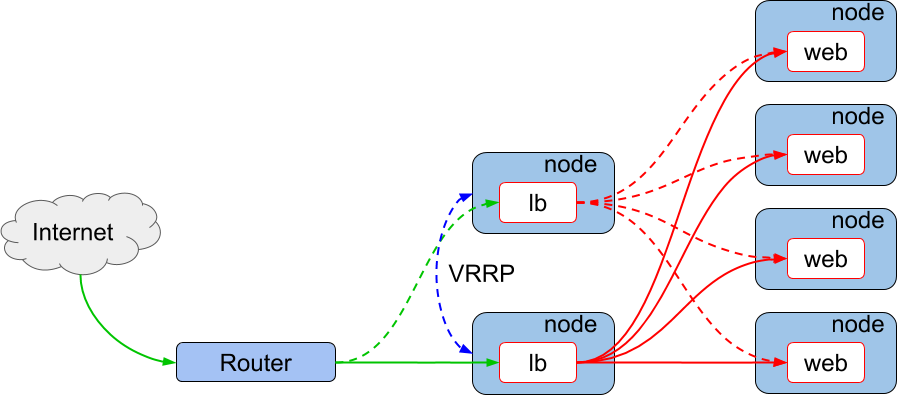
\includegraphics[width=\columnwidth]{Figs/vrrp.png}
\end{center}
\caption{ An alternative redundant load balancer architecture using VRRP.}
  The traffic from the internet is forwarded by the upstream router to a active lb node(the solid green line) and then distributed by the lb pods to web pods using Linux kernel's ipvs(the solid red line).
  The active lb pod is selected using VRRP protocol(the blue dotted line).
  For the green lines global IP address is used. The red lines use IP addresses of overlay network. The blue line uses the IP address of node network.

\label{fig:vrrp}
\end{figure}

Fig.~\ref{fig:vrrp} shows the redundancy setup using the VRRP protocol.
In the case of VRRP, the load balancer container needs to run in the node net namespace for the following two reasons;
1) When fail over occurs, the new master sends gratuitous Address Resolution Packets(ARP) packets to update the ARP cache of the upstream router and Forwarding Data Base(FDB) of layer 2 swicthes during the transition.
Such gratuitous ARP packets should consist of the virtual IP address shared by the load balancers and the MAC address of the node where the new master load balancer is running.
Programs that send out gratuitous ARP with node MAC address should be in the node net namespace.
%
2) Furthermore, the active load balancer sends out periodic advertisement using UDP multicast packet to inform existence of itself.
The load balancer in backup state stays calm unless the VRRP advertisement stops for a specified duration of time.
The UDP multicast is often unsupported in overlay network used by container cluster environment, and hence the load balancer needs to be able to use the node net namespace.
%
Running containers in the node net namespace loses the whole point of containerization, i.e., they share the node network without separation.
This requires the users' additional efforts to avoid conflict in VRRP configuration for multiple services.
%

VRRP programs also support unicast advertisement by specifying IP addresses of peer load balancers before it starts.
However, container cluster management system randomly assign IP addresses of containers when it launches them, and it is impossible to know peer IPs in advance. 
Therefore the unicast mode is not feasible in container cluster environment.

The other drawback compared with the ECMP case is that the redundancy of VRRP is provided in Active-Backup manner.
This means that a single software load balancer limits the overall performance of the entire container cluster.
Therefore we believe the ECMP redundancy is better than VRRP in our use cases.

\section{Gobgpd and zebra configurations on the router.}

{\bf\normalsize gobgp.conf:}
\begin{verbatim}
global:
  config:
    as: 65021
    router-id: 10.0.0.110
    local-address-list:
    - 0.0.0.0

  use-multiple-paths:
    config:
      enabled: true

neighbors:
    - config:
        neighbor-address: 10.0.0.109
        peer-as: 65021
      add-paths:
        config:
          receive: true

zebra:
  config:
    enabled: true
    url: unix:/run/quagga/zserv.api
    version: 3
    redistribute-route-type-list: 
      - static

\end{verbatim}
\label{appendix:router_config}

The "use-multiple-paths" should be enabled for the gobgpd to redistribute BGP multipath routes to Zebra.

\par\bigskip
\noindent {\bf\normalsize zebra.conf:}
\begin{verbatim}
hostname Router
log file /var/log/zebra.log
\end{verbatim}


\section{Gobgpd configuration on the route reflector.}
\label{appendix:route_reflector_config}

{\bf\normalsize gobgp.conf:}
\begin{verbatim}
global:
  config:
    as: 65021
    router-id: 10.0.0.109
    local-address-list:
    - 0.0.0.0 # ipv4 only
  use-multiple-paths:
    config:
      enabled: true

peer-groups:
  - config:
      peer-group-name: k8s
      peer-as: 65021
    afi-safis:
      - config:
          afi-safi-name: ipv4-unicast

dynamic-neighbors:
  - config:
      prefix: 172.16.0.0/16
      peer-group: k8s

neighbors:
  - config:
      neighbor-address: 10.0.0.110
      peer-as: 65021
    route-reflector:
      config:
        route-reflector-client: true
        route-reflector-cluster-id: 10.0.0.109
    add-paths: 
      config:
        send-max: 255
        receive: true

\end{verbatim}

The "dynamic-neighbors" section and the "peer-groups" section set up dynamic neighbor settings to avoid listing of every possible IP. 
The "add-paths" setting in the "neighbors" section enables multi path advertisement for a single network prefix.

\section{Exabgp configuration on the load balancer container.}
\label{appendix:exabgp_config}

{\bf\normalsize exabgp.conf:}
\begin{verbatim}
neighbor 10.0.0.109 {
 description "peer1";
 router-id 172.16.20.2;
 local-address 172.16.20.2;
 local-as 65021;
 peer-as 65021;
 hold-time 1800;
   static {
     route 10.1.1.0/24 next-hop 10.0.0.106;
   }
}
\end{verbatim}

The IP address of the load balancer pod(i.e. container), "172.16.20.2", is used for "router-id" and "local-address".
This address is dynamically assigned when the pod is started.
The IP address of the node, "10.0.0.106", is used for "next-hop".
The node address is found out when the pod starts.

